a. We can also define a backwards Gauss-Seidel method by setting

$$u^{[k+1]}_i=\frac12(u^{[k]}_{i-1}+u^{[k+1]}_{i+1}-h^2f_i), \text{for}\; i=m, m-1, m-2, . . . , 1$$

Show that this is a matrix splitting method of the type described in Section 4.2 with $M=D-U$ and
$N=L$.\\
b. Implement this method in \textit{iter\_bvp\_Asplit.m} and observe that it converges at the same rate
as forward Gauss-Siedel for this problem.\\\\

\begin{solution}\renewcommand{\qedsymbol}{}\ \\
    Let $M=D-U$ and $N=L$. Then, plugging these into
    
    $$Mu^{[k+1]}_i=Nu^{[k]}_i+f$$
    
    yields
    
    $$(D-U)u^{[k+1]}_i=Lu^{[k]}_i+f_i$$
    
    Hence,
    
    $$Du^{[k+1]}_i-Uu^{[k+1]}_i=Lu^{[k]}_i+f_i$$
    
    So,
    
    $$Du^{[k+1]}_i=Uu^{[k+1]}_i+Lu^{[k]}_i+f_i$$
    
    and therefore
    
    $$\frac{-2}{h^2}Iu^{[k+1]}_i=\frac{-1}{h^2}(u^{[k+1]}_{i+1}+u^{[k]}_{i-1})+f_i$$
    
    Thus,
    
    $$u^{[k+1]}_i=\frac12(u^{[k+1]}_{i+1}+u^{[k]}_{i-1}-h^2f_i)$$
    
    which is the type of splitting method desired.\\

    It is obviuos by the figures below that the the rate of convergence for the forward and the backward
    Gauss-Siedel methods is the same.
    \begin{center}
        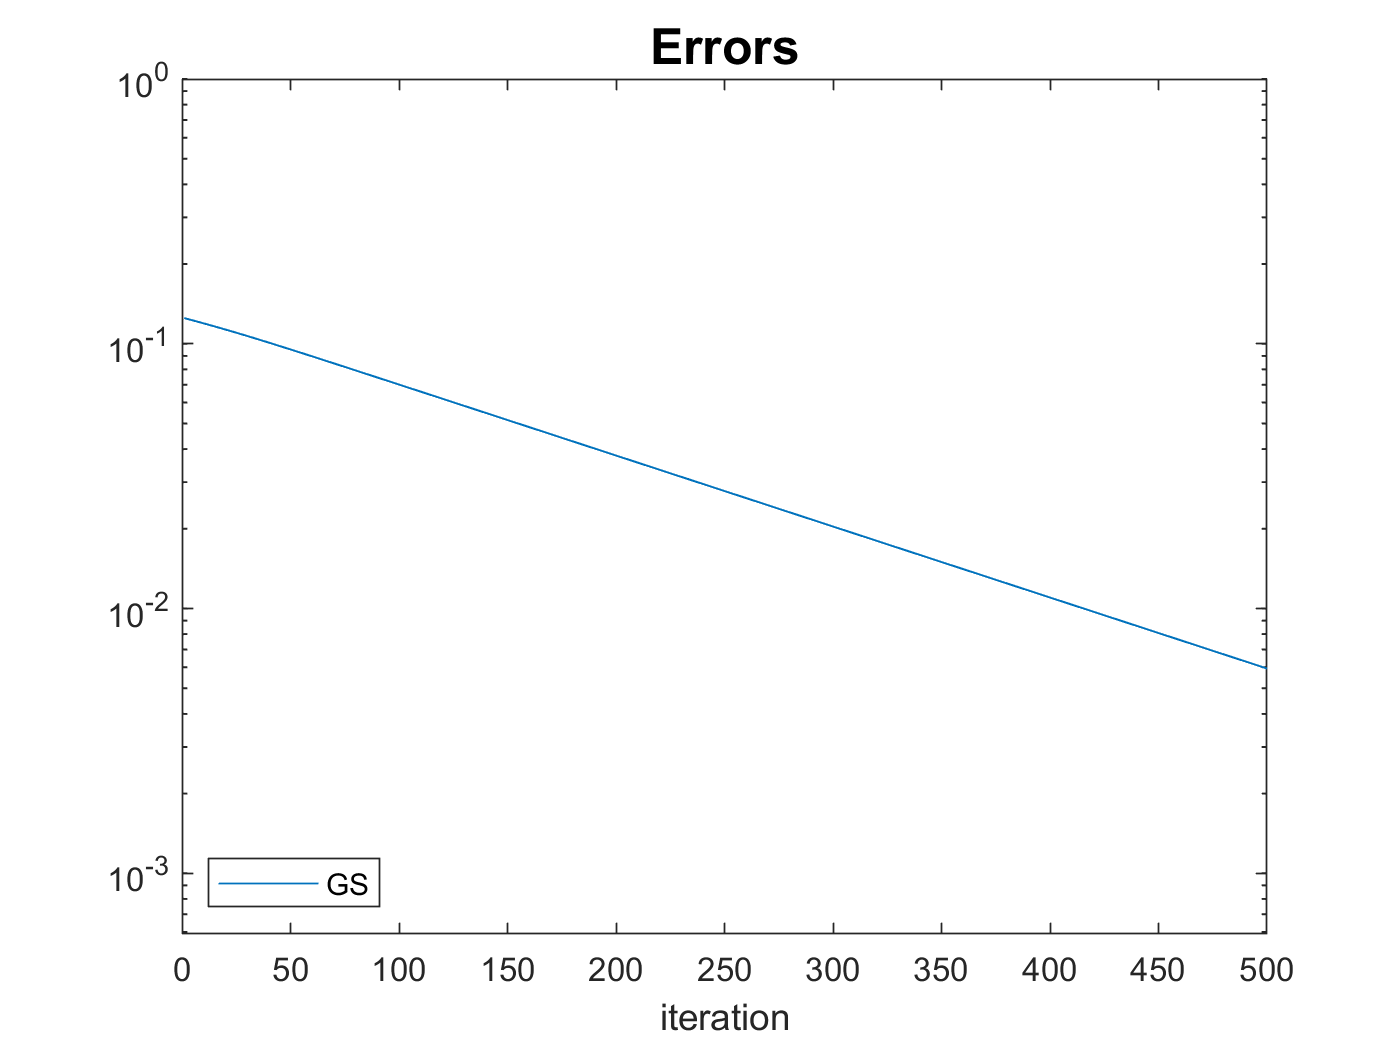
\includegraphics[scale=0.2]{gs.PNG}
    \end{center}
    \begin{center}
        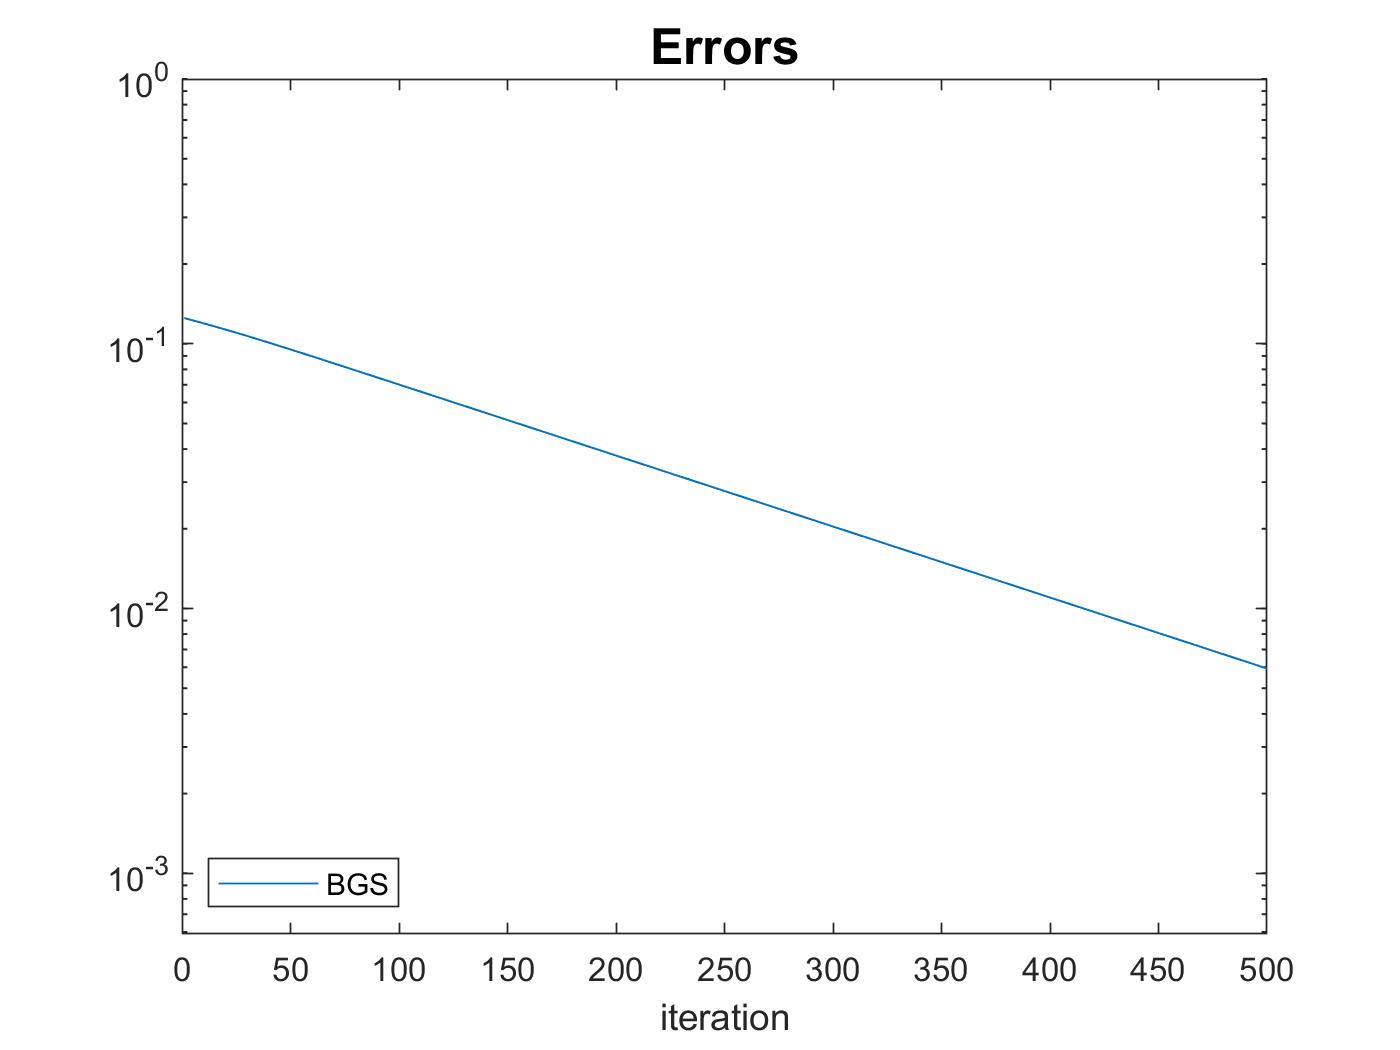
\includegraphics[scale=0.2]{bgs.PNG}
    \end{center}

\end{solution}

\newpage
\lstinputlisting{iter_bvp_Asplit.m}
\newpage
\lstinputlisting{omegaiteration.m}